% Created by tikzDevice version 0.12.3.1 on 2022-08-31 08:54:46
% !TEX encoding = UTF-8 Unicode
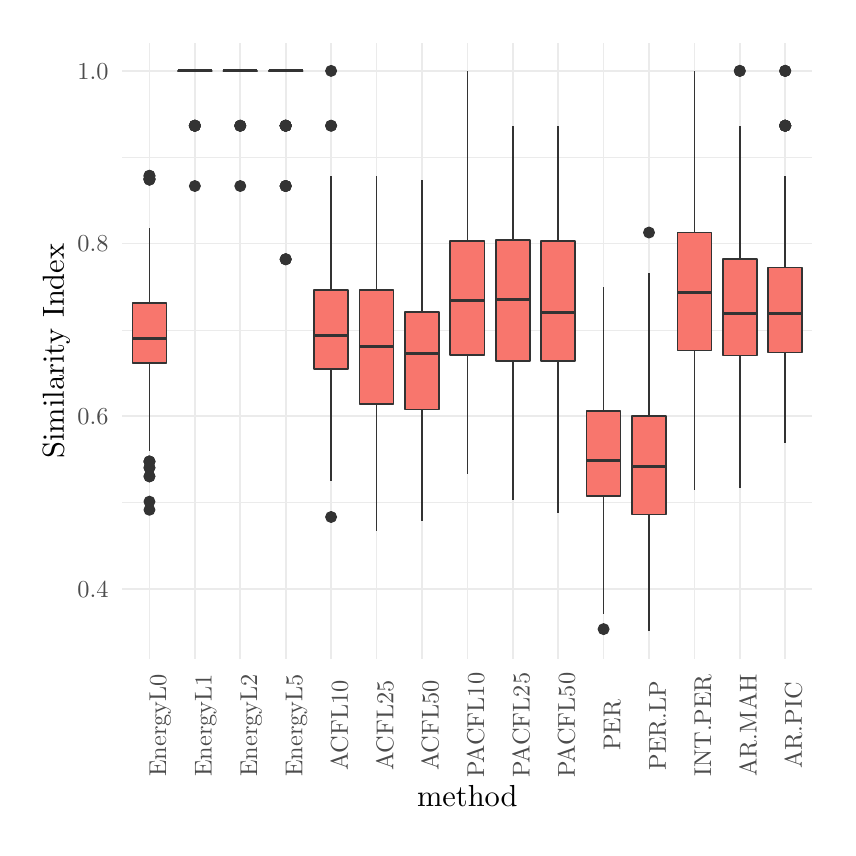
\begin{tikzpicture}[x=1pt,y=1pt]
\definecolor{fillColor}{RGB}{255,255,255}
\path[use as bounding box,fill=fillColor,fill opacity=0.00] (0,0) rectangle (289.08,289.08);
\begin{scope}
\path[clip] ( 34.16, 60.92) rectangle (283.58,283.58);
\definecolor{drawColor}{gray}{0.92}

\path[draw=drawColor,line width= 0.3pt,line join=round] ( 34.16,117.46) --
	(283.58,117.46);

\path[draw=drawColor,line width= 0.3pt,line join=round] ( 34.16,179.86) --
	(283.58,179.86);

\path[draw=drawColor,line width= 0.3pt,line join=round] ( 34.16,242.26) --
	(283.58,242.26);

\path[draw=drawColor,line width= 0.6pt,line join=round] ( 34.16, 86.27) --
	(283.58, 86.27);

\path[draw=drawColor,line width= 0.6pt,line join=round] ( 34.16,148.66) --
	(283.58,148.66);

\path[draw=drawColor,line width= 0.6pt,line join=round] ( 34.16,211.06) --
	(283.58,211.06);

\path[draw=drawColor,line width= 0.6pt,line join=round] ( 34.16,273.46) --
	(283.58,273.46);

\path[draw=drawColor,line width= 0.6pt,line join=round] ( 44.00, 60.92) --
	( 44.00,283.58);

\path[draw=drawColor,line width= 0.6pt,line join=round] ( 60.41, 60.92) --
	( 60.41,283.58);

\path[draw=drawColor,line width= 0.6pt,line join=round] ( 76.82, 60.92) --
	( 76.82,283.58);

\path[draw=drawColor,line width= 0.6pt,line join=round] ( 93.23, 60.92) --
	( 93.23,283.58);

\path[draw=drawColor,line width= 0.6pt,line join=round] (109.64, 60.92) --
	(109.64,283.58);

\path[draw=drawColor,line width= 0.6pt,line join=round] (126.05, 60.92) --
	(126.05,283.58);

\path[draw=drawColor,line width= 0.6pt,line join=round] (142.46, 60.92) --
	(142.46,283.58);

\path[draw=drawColor,line width= 0.6pt,line join=round] (158.87, 60.92) --
	(158.87,283.58);

\path[draw=drawColor,line width= 0.6pt,line join=round] (175.28, 60.92) --
	(175.28,283.58);

\path[draw=drawColor,line width= 0.6pt,line join=round] (191.69, 60.92) --
	(191.69,283.58);

\path[draw=drawColor,line width= 0.6pt,line join=round] (208.10, 60.92) --
	(208.10,283.58);

\path[draw=drawColor,line width= 0.6pt,line join=round] (224.51, 60.92) --
	(224.51,283.58);

\path[draw=drawColor,line width= 0.6pt,line join=round] (240.92, 60.92) --
	(240.92,283.58);

\path[draw=drawColor,line width= 0.6pt,line join=round] (257.32, 60.92) --
	(257.32,283.58);

\path[draw=drawColor,line width= 0.6pt,line join=round] (273.73, 60.92) --
	(273.73,283.58);
\definecolor{drawColor}{gray}{0.20}
\definecolor{fillColor}{gray}{0.20}

\path[draw=drawColor,line width= 0.4pt,line join=round,line cap=round,fill=fillColor] ( 44.00,114.86) circle (  1.96);

\path[draw=drawColor,line width= 0.4pt,line join=round,line cap=round,fill=fillColor] ( 44.00,126.94) circle (  1.96);

\path[draw=drawColor,line width= 0.4pt,line join=round,line cap=round,fill=fillColor] ( 44.00,234.46) circle (  1.96);

\path[draw=drawColor,line width= 0.4pt,line join=round,line cap=round,fill=fillColor] ( 44.00,234.15) circle (  1.96);

\path[draw=drawColor,line width= 0.4pt,line join=round,line cap=round,fill=fillColor] ( 44.00,234.46) circle (  1.96);

\path[draw=drawColor,line width= 0.4pt,line join=round,line cap=round,fill=fillColor] ( 44.00,234.46) circle (  1.96);

\path[draw=drawColor,line width= 0.4pt,line join=round,line cap=round,fill=fillColor] ( 44.00,130.09) circle (  1.96);

\path[draw=drawColor,line width= 0.4pt,line join=round,line cap=round,fill=fillColor] ( 44.00,132.32) circle (  1.96);

\path[draw=drawColor,line width= 0.4pt,line join=round,line cap=round,fill=fillColor] ( 44.00,132.32) circle (  1.96);

\path[draw=drawColor,line width= 0.4pt,line join=round,line cap=round,fill=fillColor] ( 44.00,235.57) circle (  1.96);

\path[draw=drawColor,line width= 0.4pt,line join=round,line cap=round,fill=fillColor] ( 44.00,126.94) circle (  1.96);

\path[draw=drawColor,line width= 0.4pt,line join=round,line cap=round,fill=fillColor] ( 44.00,132.32) circle (  1.96);

\path[draw=drawColor,line width= 0.4pt,line join=round,line cap=round,fill=fillColor] ( 44.00,117.81) circle (  1.96);

\path[draw=drawColor,line width= 0.4pt,line join=round,line cap=round,fill=fillColor] ( 44.00,234.15) circle (  1.96);

\path[draw=drawColor,line width= 0.4pt,line join=round,line cap=round,fill=fillColor] ( 44.00,235.57) circle (  1.96);

\path[draw=drawColor,line width= 0.4pt,line join=round,line cap=round,fill=fillColor] ( 44.00,130.09) circle (  1.96);

\path[draw=drawColor,line width= 0.6pt,line join=round] ( 44.00,189.52) -- ( 44.00,216.82);

\path[draw=drawColor,line width= 0.6pt,line join=round] ( 44.00,167.99) -- ( 44.00,136.04);
\definecolor{fillColor}{RGB}{248,118,109}

\path[draw=drawColor,line width= 0.6pt,line join=round,line cap=round,fill=fillColor] ( 37.85,189.52) --
	( 37.85,167.99) --
	( 50.16,167.99) --
	( 50.16,189.52) --
	( 37.85,189.52) --
	cycle;

\path[draw=drawColor,line width= 1.1pt,line join=round] ( 37.85,176.89) -- ( 50.16,176.89);
\definecolor{fillColor}{gray}{0.20}

\path[draw=drawColor,line width= 0.4pt,line join=round,line cap=round,fill=fillColor] ( 60.41,253.65) circle (  1.96);

\path[draw=drawColor,line width= 0.4pt,line join=round,line cap=round,fill=fillColor] ( 60.41,253.65) circle (  1.96);

\path[draw=drawColor,line width= 0.4pt,line join=round,line cap=round,fill=fillColor] ( 60.41,253.65) circle (  1.96);

\path[draw=drawColor,line width= 0.4pt,line join=round,line cap=round,fill=fillColor] ( 60.41,231.86) circle (  1.96);

\path[draw=drawColor,line width= 0.4pt,line join=round,line cap=round,fill=fillColor] ( 60.41,253.65) circle (  1.96);

\path[draw=drawColor,line width= 0.4pt,line join=round,line cap=round,fill=fillColor] ( 60.41,253.65) circle (  1.96);

\path[draw=drawColor,line width= 0.4pt,line join=round,line cap=round,fill=fillColor] ( 60.41,253.65) circle (  1.96);

\path[draw=drawColor,line width= 0.6pt,line join=round] ( 60.41,273.46) -- ( 60.41,273.46);

\path[draw=drawColor,line width= 0.6pt,line join=round] ( 60.41,273.46) -- ( 60.41,273.46);
\definecolor{fillColor}{RGB}{248,118,109}

\path[draw=drawColor,line width= 0.6pt,line join=round,line cap=round,fill=fillColor] ( 54.26,273.46) --
	( 54.26,273.46) --
	( 66.56,273.46) --
	( 66.56,273.46) --
	( 54.26,273.46) --
	cycle;

\path[draw=drawColor,line width= 1.1pt,line join=round] ( 54.26,273.46) -- ( 66.56,273.46);
\definecolor{fillColor}{gray}{0.20}

\path[draw=drawColor,line width= 0.4pt,line join=round,line cap=round,fill=fillColor] ( 76.82,253.65) circle (  1.96);

\path[draw=drawColor,line width= 0.4pt,line join=round,line cap=round,fill=fillColor] ( 76.82,231.86) circle (  1.96);

\path[draw=drawColor,line width= 0.4pt,line join=round,line cap=round,fill=fillColor] ( 76.82,253.65) circle (  1.96);

\path[draw=drawColor,line width= 0.4pt,line join=round,line cap=round,fill=fillColor] ( 76.82,253.65) circle (  1.96);

\path[draw=drawColor,line width= 0.4pt,line join=round,line cap=round,fill=fillColor] ( 76.82,253.65) circle (  1.96);

\path[draw=drawColor,line width= 0.6pt,line join=round] ( 76.82,273.46) -- ( 76.82,273.46);

\path[draw=drawColor,line width= 0.6pt,line join=round] ( 76.82,273.46) -- ( 76.82,273.46);
\definecolor{fillColor}{RGB}{248,118,109}

\path[draw=drawColor,line width= 0.6pt,line join=round,line cap=round,fill=fillColor] ( 70.67,273.46) --
	( 70.67,273.46) --
	( 82.97,273.46) --
	( 82.97,273.46) --
	( 70.67,273.46) --
	cycle;

\path[draw=drawColor,line width= 1.1pt,line join=round] ( 70.67,273.46) -- ( 82.97,273.46);
\definecolor{fillColor}{gray}{0.20}

\path[draw=drawColor,line width= 0.4pt,line join=round,line cap=round,fill=fillColor] ( 93.23,253.65) circle (  1.96);

\path[draw=drawColor,line width= 0.4pt,line join=round,line cap=round,fill=fillColor] ( 93.23,231.86) circle (  1.96);

\path[draw=drawColor,line width= 0.4pt,line join=round,line cap=round,fill=fillColor] ( 93.23,205.39) circle (  1.96);

\path[draw=drawColor,line width= 0.4pt,line join=round,line cap=round,fill=fillColor] ( 93.23,253.65) circle (  1.96);

\path[draw=drawColor,line width= 0.4pt,line join=round,line cap=round,fill=fillColor] ( 93.23,205.39) circle (  1.96);

\path[draw=drawColor,line width= 0.4pt,line join=round,line cap=round,fill=fillColor] ( 93.23,253.65) circle (  1.96);

\path[draw=drawColor,line width= 0.4pt,line join=round,line cap=round,fill=fillColor] ( 93.23,253.65) circle (  1.96);

\path[draw=drawColor,line width= 0.4pt,line join=round,line cap=round,fill=fillColor] ( 93.23,253.65) circle (  1.96);

\path[draw=drawColor,line width= 0.4pt,line join=round,line cap=round,fill=fillColor] ( 93.23,253.65) circle (  1.96);

\path[draw=drawColor,line width= 0.4pt,line join=round,line cap=round,fill=fillColor] ( 93.23,231.86) circle (  1.96);

\path[draw=drawColor,line width= 0.4pt,line join=round,line cap=round,fill=fillColor] ( 93.23,231.86) circle (  1.96);

\path[draw=drawColor,line width= 0.4pt,line join=round,line cap=round,fill=fillColor] ( 93.23,253.65) circle (  1.96);

\path[draw=drawColor,line width= 0.4pt,line join=round,line cap=round,fill=fillColor] ( 93.23,253.65) circle (  1.96);

\path[draw=drawColor,line width= 0.4pt,line join=round,line cap=round,fill=fillColor] ( 93.23,253.65) circle (  1.96);

\path[draw=drawColor,line width= 0.4pt,line join=round,line cap=round,fill=fillColor] ( 93.23,231.86) circle (  1.96);

\path[draw=drawColor,line width= 0.4pt,line join=round,line cap=round,fill=fillColor] ( 93.23,205.39) circle (  1.96);

\path[draw=drawColor,line width= 0.6pt,line join=round] ( 93.23,273.46) -- ( 93.23,273.46);

\path[draw=drawColor,line width= 0.6pt,line join=round] ( 93.23,273.46) -- ( 93.23,273.46);
\definecolor{fillColor}{RGB}{248,118,109}

\path[draw=drawColor,line width= 0.6pt,line join=round,line cap=round,fill=fillColor] ( 87.08,273.46) --
	( 87.08,273.46) --
	( 99.38,273.46) --
	( 99.38,273.46) --
	( 87.08,273.46) --
	cycle;

\path[draw=drawColor,line width= 1.1pt,line join=round] ( 87.08,273.46) -- ( 99.38,273.46);
\definecolor{fillColor}{gray}{0.20}

\path[draw=drawColor,line width= 0.4pt,line join=round,line cap=round,fill=fillColor] (109.64,253.65) circle (  1.96);

\path[draw=drawColor,line width= 0.4pt,line join=round,line cap=round,fill=fillColor] (109.64,253.65) circle (  1.96);

\path[draw=drawColor,line width= 0.4pt,line join=round,line cap=round,fill=fillColor] (109.64,273.46) circle (  1.96);

\path[draw=drawColor,line width= 0.4pt,line join=round,line cap=round,fill=fillColor] (109.64,112.26) circle (  1.96);

\path[draw=drawColor,line width= 0.6pt,line join=round] (109.64,194.22) -- (109.64,235.57);

\path[draw=drawColor,line width= 0.6pt,line join=round] (109.64,165.78) -- (109.64,125.16);
\definecolor{fillColor}{RGB}{248,118,109}

\path[draw=drawColor,line width= 0.6pt,line join=round,line cap=round,fill=fillColor] (103.49,194.22) --
	(103.49,165.78) --
	(115.79,165.78) --
	(115.79,194.22) --
	(103.49,194.22) --
	cycle;

\path[draw=drawColor,line width= 1.1pt,line join=round] (103.49,177.76) -- (115.79,177.76);

\path[draw=drawColor,line width= 0.6pt,line join=round] (126.05,194.22) -- (126.05,235.57);

\path[draw=drawColor,line width= 0.6pt,line join=round] (126.05,153.12) -- (126.05,107.06);

\path[draw=drawColor,line width= 0.6pt,line join=round,line cap=round,fill=fillColor] (119.90,194.22) --
	(119.90,153.12) --
	(132.20,153.12) --
	(132.20,194.22) --
	(119.90,194.22) --
	cycle;

\path[draw=drawColor,line width= 1.1pt,line join=round] (119.90,173.98) -- (132.20,173.98);

\path[draw=drawColor,line width= 0.6pt,line join=round] (142.46,186.36) -- (142.46,234.15);

\path[draw=drawColor,line width= 0.6pt,line join=round] (142.46,151.09) -- (142.46,110.96);

\path[draw=drawColor,line width= 0.6pt,line join=round,line cap=round,fill=fillColor] (136.31,186.36) --
	(136.31,151.09) --
	(148.61,151.09) --
	(148.61,186.36) --
	(136.31,186.36) --
	cycle;

\path[draw=drawColor,line width= 1.1pt,line join=round] (136.31,171.35) -- (148.61,171.35);

\path[draw=drawColor,line width= 0.6pt,line join=round] (158.87,211.91) -- (158.87,273.46);

\path[draw=drawColor,line width= 0.6pt,line join=round] (158.87,170.74) -- (158.87,127.76);

\path[draw=drawColor,line width= 0.6pt,line join=round,line cap=round,fill=fillColor] (152.71,211.91) --
	(152.71,170.74) --
	(165.02,170.74) --
	(165.02,211.91) --
	(152.71,211.91) --
	cycle;

\path[draw=drawColor,line width= 1.1pt,line join=round] (152.71,190.63) -- (165.02,190.63);

\path[draw=drawColor,line width= 0.6pt,line join=round] (175.28,212.24) -- (175.28,253.65);

\path[draw=drawColor,line width= 0.6pt,line join=round] (175.28,168.72) -- (175.28,118.33);

\path[draw=drawColor,line width= 0.6pt,line join=round,line cap=round,fill=fillColor] (169.12,212.24) --
	(169.12,168.72) --
	(181.43,168.72) --
	(181.43,212.24) --
	(169.12,212.24) --
	cycle;

\path[draw=drawColor,line width= 1.1pt,line join=round] (169.12,191.00) -- (181.43,191.00);

\path[draw=drawColor,line width= 0.6pt,line join=round] (191.69,212.05) -- (191.69,253.65);

\path[draw=drawColor,line width= 0.6pt,line join=round] (191.69,168.72) -- (191.69,113.58);

\path[draw=drawColor,line width= 0.6pt,line join=round,line cap=round,fill=fillColor] (185.53,212.05) --
	(185.53,168.72) --
	(197.84,168.72) --
	(197.84,212.05) --
	(185.53,212.05) --
	cycle;

\path[draw=drawColor,line width= 1.1pt,line join=round] (185.53,186.13) -- (197.84,186.13);
\definecolor{fillColor}{gray}{0.20}

\path[draw=drawColor,line width= 0.4pt,line join=round,line cap=round,fill=fillColor] (208.10, 71.75) circle (  1.96);

\path[draw=drawColor,line width= 0.6pt,line join=round] (208.10,150.61) -- (208.10,195.55);

\path[draw=drawColor,line width= 0.6pt,line join=round] (208.10,119.87) -- (208.10, 77.35);
\definecolor{fillColor}{RGB}{248,118,109}

\path[draw=drawColor,line width= 0.6pt,line join=round,line cap=round,fill=fillColor] (201.94,150.61) --
	(201.94,119.87) --
	(214.25,119.87) --
	(214.25,150.61) --
	(201.94,150.61) --
	cycle;

\path[draw=drawColor,line width= 1.1pt,line join=round] (201.94,132.69) -- (214.25,132.69);
\definecolor{fillColor}{gray}{0.20}

\path[draw=drawColor,line width= 0.4pt,line join=round,line cap=round,fill=fillColor] (224.51,215.05) circle (  1.96);

\path[draw=drawColor,line width= 0.6pt,line join=round] (224.51,148.78) -- (224.51,200.48);

\path[draw=drawColor,line width= 0.6pt,line join=round] (224.51,113.21) -- (224.51, 71.04);
\definecolor{fillColor}{RGB}{248,118,109}

\path[draw=drawColor,line width= 0.6pt,line join=round,line cap=round,fill=fillColor] (218.35,148.78) --
	(218.35,113.21) --
	(230.66,113.21) --
	(230.66,148.78) --
	(218.35,148.78) --
	cycle;

\path[draw=drawColor,line width= 1.1pt,line join=round] (218.35,130.46) -- (230.66,130.46);

\path[draw=drawColor,line width= 0.6pt,line join=round] (240.92,215.05) -- (240.92,273.46);

\path[draw=drawColor,line width= 0.6pt,line join=round] (240.92,172.43) -- (240.92,122.19);

\path[draw=drawColor,line width= 0.6pt,line join=round,line cap=round,fill=fillColor] (234.76,215.05) --
	(234.76,172.43) --
	(247.07,172.43) --
	(247.07,215.05) --
	(234.76,215.05) --
	cycle;

\path[draw=drawColor,line width= 1.1pt,line join=round] (234.76,193.30) -- (247.07,193.30);
\definecolor{fillColor}{gray}{0.20}

\path[draw=drawColor,line width= 0.4pt,line join=round,line cap=round,fill=fillColor] (257.32,273.46) circle (  1.96);

\path[draw=drawColor,line width= 0.4pt,line join=round,line cap=round,fill=fillColor] (257.32,273.46) circle (  1.96);

\path[draw=drawColor,line width= 0.6pt,line join=round] (257.32,205.39) -- (257.32,253.65);

\path[draw=drawColor,line width= 0.6pt,line join=round] (257.32,170.61) -- (257.32,122.66);
\definecolor{fillColor}{RGB}{248,118,109}

\path[draw=drawColor,line width= 0.6pt,line join=round,line cap=round,fill=fillColor] (251.17,205.39) --
	(251.17,170.61) --
	(263.48,170.61) --
	(263.48,205.39) --
	(251.17,205.39) --
	cycle;

\path[draw=drawColor,line width= 1.1pt,line join=round] (251.17,185.89) -- (263.48,185.89);
\definecolor{fillColor}{gray}{0.20}

\path[draw=drawColor,line width= 0.4pt,line join=round,line cap=round,fill=fillColor] (273.73,253.65) circle (  1.96);

\path[draw=drawColor,line width= 0.4pt,line join=round,line cap=round,fill=fillColor] (273.73,273.46) circle (  1.96);

\path[draw=drawColor,line width= 0.4pt,line join=round,line cap=round,fill=fillColor] (273.73,253.65) circle (  1.96);

\path[draw=drawColor,line width= 0.4pt,line join=round,line cap=round,fill=fillColor] (273.73,253.65) circle (  1.96);

\path[draw=drawColor,line width= 0.4pt,line join=round,line cap=round,fill=fillColor] (273.73,253.65) circle (  1.96);

\path[draw=drawColor,line width= 0.4pt,line join=round,line cap=round,fill=fillColor] (273.73,273.46) circle (  1.96);

\path[draw=drawColor,line width= 0.4pt,line join=round,line cap=round,fill=fillColor] (273.73,253.65) circle (  1.96);

\path[draw=drawColor,line width= 0.4pt,line join=round,line cap=round,fill=fillColor] (273.73,253.65) circle (  1.96);

\path[draw=drawColor,line width= 0.4pt,line join=round,line cap=round,fill=fillColor] (273.73,253.65) circle (  1.96);

\path[draw=drawColor,line width= 0.4pt,line join=round,line cap=round,fill=fillColor] (273.73,253.65) circle (  1.96);

\path[draw=drawColor,line width= 0.4pt,line join=round,line cap=round,fill=fillColor] (273.73,273.46) circle (  1.96);

\path[draw=drawColor,line width= 0.6pt,line join=round] (273.73,202.39) -- (273.73,235.57);

\path[draw=drawColor,line width= 0.6pt,line join=round] (273.73,171.66) -- (273.73,139.13);
\definecolor{fillColor}{RGB}{248,118,109}

\path[draw=drawColor,line width= 0.6pt,line join=round,line cap=round,fill=fillColor] (267.58,202.39) --
	(267.58,171.66) --
	(279.89,171.66) --
	(279.89,202.39) --
	(267.58,202.39) --
	cycle;

\path[draw=drawColor,line width= 1.1pt,line join=round] (267.58,185.89) -- (279.89,185.89);
\end{scope}
\begin{scope}
\path[clip] (  0.00,  0.00) rectangle (289.08,289.08);
\definecolor{drawColor}{gray}{0.30}

\node[text=drawColor,anchor=base east,inner sep=0pt, outer sep=0pt, scale=  0.88] at ( 29.21, 83.24) {0.4};

\node[text=drawColor,anchor=base east,inner sep=0pt, outer sep=0pt, scale=  0.88] at ( 29.21,145.63) {0.6};

\node[text=drawColor,anchor=base east,inner sep=0pt, outer sep=0pt, scale=  0.88] at ( 29.21,208.03) {0.8};

\node[text=drawColor,anchor=base east,inner sep=0pt, outer sep=0pt, scale=  0.88] at ( 29.21,270.43) {1.0};
\end{scope}
\begin{scope}
\path[clip] (  0.00,  0.00) rectangle (289.08,289.08);
\definecolor{drawColor}{gray}{0.30}

\node[text=drawColor,rotate= 90.00,anchor=base,inner sep=0pt, outer sep=0pt, scale=  0.88] at ( 50.06, 36.97) {EnergyL0};

\node[text=drawColor,rotate= 90.00,anchor=base,inner sep=0pt, outer sep=0pt, scale=  0.88] at ( 66.47, 36.97) {EnergyL1};

\node[text=drawColor,rotate= 90.00,anchor=base,inner sep=0pt, outer sep=0pt, scale=  0.88] at ( 82.88, 36.97) {EnergyL2};

\node[text=drawColor,rotate= 90.00,anchor=base,inner sep=0pt, outer sep=0pt, scale=  0.88] at ( 99.29, 36.97) {EnergyL5};

\node[text=drawColor,rotate= 90.00,anchor=base,inner sep=0pt, outer sep=0pt, scale=  0.88] at (115.70, 36.97) {ACFL10};

\node[text=drawColor,rotate= 90.00,anchor=base,inner sep=0pt, outer sep=0pt, scale=  0.88] at (132.11, 36.97) {ACFL25};

\node[text=drawColor,rotate= 90.00,anchor=base,inner sep=0pt, outer sep=0pt, scale=  0.88] at (148.52, 36.97) {ACFL50};

\node[text=drawColor,rotate= 90.00,anchor=base,inner sep=0pt, outer sep=0pt, scale=  0.88] at (164.93, 36.97) {PACFL10};

\node[text=drawColor,rotate= 90.00,anchor=base,inner sep=0pt, outer sep=0pt, scale=  0.88] at (181.34, 36.97) {PACFL25};

\node[text=drawColor,rotate= 90.00,anchor=base,inner sep=0pt, outer sep=0pt, scale=  0.88] at (197.75, 36.97) {PACFL50};

\node[text=drawColor,rotate= 90.00,anchor=base,inner sep=0pt, outer sep=0pt, scale=  0.88] at (214.16, 36.97) {PER};

\node[text=drawColor,rotate= 90.00,anchor=base,inner sep=0pt, outer sep=0pt, scale=  0.88] at (230.57, 36.97) {PER.LP};

\node[text=drawColor,rotate= 90.00,anchor=base,inner sep=0pt, outer sep=0pt, scale=  0.88] at (246.98, 36.97) {INT.PER};

\node[text=drawColor,rotate= 90.00,anchor=base,inner sep=0pt, outer sep=0pt, scale=  0.88] at (263.39, 36.97) {AR.MAH};

\node[text=drawColor,rotate= 90.00,anchor=base,inner sep=0pt, outer sep=0pt, scale=  0.88] at (279.80, 36.97) {AR.PIC};
\end{scope}
\begin{scope}
\path[clip] (  0.00,  0.00) rectangle (289.08,289.08);
\definecolor{drawColor}{RGB}{0,0,0}

\node[text=drawColor,anchor=base,inner sep=0pt, outer sep=0pt, scale=  1.10] at (158.87,  7.64) {method};
\end{scope}
\begin{scope}
\path[clip] (  0.00,  0.00) rectangle (289.08,289.08);
\definecolor{drawColor}{RGB}{0,0,0}

\node[text=drawColor,rotate= 90.00,anchor=base,inner sep=0pt, outer sep=0pt, scale=  1.10] at ( 13.08,172.25) {Similarity Index};
\end{scope}
\end{tikzpicture}
